%Symbole

% Symbol: Pfeil zum Zurückspringen
\newcommand{\zurueck}{%
	\begin{tikzpicture}[scale=0.15]
%	\fill [gray!40] (0,0) circle [radius=1.5];
	\draw [thick, -{>[length=3pt, width=5pt]}] (-0.6,0.6) arc [start angle=-230, end angle=100, radius=1] -- ++(-0.1,0);
	\end{tikzpicture}
}

%Symbol: Werkzeug
\newcommand{\werkzeug}{%
	
\begin{tikzpicture}[scale=0.1, rotate=45]
%	\filldraw [fill=white, draw=black] (3,0) circle [radius=4cm];
	\path [thick, fill=gray, draw=black] (3.5,0.5) -- (0,0.5) arc [start angle=90, end angle=270, radius=0.5] (0,-0.5) -- (3.5,-0.5) -- (3.8,0) -- (3.5,0.5);
	\path [thick,draw=black, fill=gray] (3.5,-0.5) ++(1,0.5) ++(206.57:1.118) arc (206.57:315:1.118) -- ++(-0.9,0) -- (3.8,0) ++ (0.7,0) ++(-206.57:1.118) arc (-206.57:-315:1.118) -- ++(-0.9,0) -- (3.8,0);
	\draw [very thick, gray] (3.5,-0.5) -- (3.8,0) -- (3.5,0.5);
	\fill [gray!50, rounded corners=1] (0.3,0.25) rectangle (3.2,0.3);
	\fill [gray!50, rounded corners=1] (0.3,-0.25) rectangle (3.2,-0.3);
	\end{tikzpicture}
}

%Symbol: Drucker
\newcommand{\drucker}{%
	
\begin{tikzpicture}[scale=0.2]
		\draw (0.5,0.5) rectangle (1.5,1.8);
		\foreach \x in {1.2,1.4,1.6}	
		\draw (0.6,\x) -- (1.4,\x);
		\draw [rounded corners=0.5pt, fill=gray!80!black] (0,0) rectangle (2,1);
	\end{tikzpicture}
}

%Symbol: Video
\newcommand{\video}{%
	
\begin{tikzpicture}[scale=0.2]
		\draw [rounded corners=3pt, fill=gray!20] (0,0) rectangle (3,2);
		\draw [fill=gray] (1,0.5) -- (1,1.5) -- (2,1) -- (1,0.5);
	\end{tikzpicture}
}

%Symbol: Präsentationsfolie
\newcommand{\folie}{%
	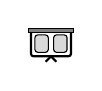
\begin{tikzpicture}[scale=0.17]
	\draw [rounded corners=1pt,thick] (0,0) rectangle (3,2);
	\draw [rounded corners=1pt,fill=gray!30] (0.3,0.3) rectangle (1.3,1.6);
	\draw [rounded corners=1pt,fill=gray!30] (1.7,0.3) rectangle (2.7,1.6);
	\draw [thick] (1.1,-0.4) -- (1.5,0) -- (1.9,-0.4);
	\draw [fill=gray] (-0.2,1.8) rectangle (3.2,2.1);
	\end{tikzpicture}
}

%Symbol: Internetlink
\newcommand{\wlan}{%
	
\begin{tikzpicture}[scale=0.5]
		\fill[black] (1mm,1mm) circle [radius=1mm];
		\draw [ultra thick] (0.4,0) arc [start angle=0, end angle=90, radius=4mm];
		\draw [ultra thick] (0.6,0) arc [start angle=0, end angle=90, radius=6mm];
		\draw [ultra thick] (0.8,0) arc [start angle=0, end angle=90, radius=8mm];
	\end{tikzpicture}
}

%Symbol: Ausrufezeichen
\newcommand{\ausrufezeichen}{%
	
\begin{tikzpicture}[scale=0.8]
	\fill[gray!70] (0,0) circle [radius=1mm];
	\fill[gray] (0,0.15) -- (0.05,0.6) -- (-0.25,0.7) -- (-0.1,0.15) -- (0,0.15);
	\fill[gray!50] (0.05,0.15) -- (0.1,0.6) -- (-0.2,0.7) -- (-0.05,0.15) -- (0.05,0.15);
	\end{tikzpicture}
}

%Symbol: Schaltplan
\newcommand{\schaltsym}{%
	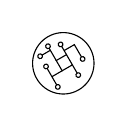
\begin{tikzpicture}[scale=0.3,rotate=30]
		\filldraw [fill=white, draw=black] (0.2,0.25) circle [radius=1.3];
		\draw (0,0) rectangle (0.5,0.5);
		\draw (0,0.5) -- (0,1.2) (0,1) -- (-0.5,1);
		\filldraw [fill=white, draw=black] (0,1.2) circle [radius=0.1];
		\filldraw [fill=white, draw=black] (-0.5,1) circle [radius=0.1];
		\draw (0.5,0.5) -- (0.5,1) (0.5,0.7) -- (1,0.7) -- (1,0);
		\filldraw [fill=white, draw=black] (0.5,1) circle [radius=0.1];
		\filldraw [fill=white, draw=black] (1,0) circle [radius=0.1];
		%\draw (1,0.5) -- (1,1) (1,0.5) -- (1.5,0.5) -- (1.5,1);
		%\filldraw [fill=white, draw=black] (1,1) circle [radius=0.1];
		%\filldraw [fill=white, draw=black] (1.5,1) circle [radius=0.1];
		%\draw (1,0) -- (1.5,0) -- (1.5,-0.5);
		%\filldraw [fill=white, draw=black] (1.5,-0.5) circle [radius=0.1];
		\draw (0.5,0) -- (0.5,-0.5);
		\filldraw [fill=white, draw=black] (0.5,-0.5) circle [radius=0.1];
		\draw (0,0) -- (-0.5,0) (-0.5,0.5) -- (-0.5,-0.5);
		\filldraw [fill=white, draw=black] (-0.5,0.5) circle [radius=0.1];
		\filldraw [fill=white, draw=black] (-0.5,-0.5) circle [radius=0.1];
	\end{tikzpicture}
}

%Symbol: Arduino / Code

\newcommand{\codesym}{%
	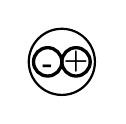
\begin{tikzpicture}[scale=0.6]
		\filldraw [thick, fill=white, draw=black] (0,0) circle [radius=0.7];
		\draw [very thick] (-0.3,0) circle [radius=0.3];
		\draw [very thick] (0.3,0) circle [radius=0.3];
		%\draw [ultra thick] (-0.1,-0.2) -- (0.1,0.2);
		%\draw [ultra thick] (-0.1,0.2) -- (0.1,-0.2);
		\node at (-0.3,-0.1) {\bfseries -};
		\node at (0.3,0) {\bfseries +};
	\end{tikzpicture}	
}

%Symbol: Lupe für eigene Untersuchungen
\newcommand{\lupe}{%
	\begin{tikzpicture}[scale=0.25]%
%	\filldraw [fill=white, draw=black] (0.6,0.6) circle [radius=1.52];
	\shadedraw [ball color=gray!10, draw=black, thick, name path=kreis] (1,1) circle (0.5);
	\path [name path=mpursprung] (1,1) -- (0,0);
	\draw [name intersections={of=kreis and mpursprung, by=x}][thick] (x) -- (0,0);
	\end{tikzpicture}%
}

%Symbol: kleines i für Informationen
\newcommand{\infosym}{%
	
\begin{tikzpicture}[scale=0.3]%
	\filldraw [fill=white, draw=black] (0,0) circle [radius=1];
	\node at (0,0) {\bfseries\LARGE i};
	\end{tikzpicture}%
}

%LED
\newcommand{\ledsym}[1][~]{%
	\begin{tikzpicture}[scale=0.7,baseline=-2mm]
	\fill [CadetBlue!70!green] (0,0) circle (0.25cm); %ursprünglich gray!50!white
	\fill [CadetBlue!70!green] (-0.25,0) rectangle (0.25,-0.3);
	\draw [thick, gray!50!white] (-0.1,-0.3) -- (-0.1,-0.4);
	\draw [thick, gray!50!white] (0.1,-0.3) -- (0.1,-0.5);
	\node at (0,-0.05) {\sffamily \bfseries #1};
	\end{tikzpicture}
}

%kleiner Widerstand
\newcommand{\resistorsym}{%
	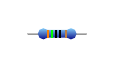
\begin{tikzpicture}[scale=0.05,baseline=-1mm]
	\shade [top color=lightgray, bottom color=gray] (-5,0.8) rectangle (10,1.2);
	\shade [top color=LightSkyBlue, bottom color=NavyBlue] (0,0) -- (5,0) arc [start angle=-135, end angle=135, radius=1.414] -- (0,2) arc [start angle=45, end angle=315, radius=1.414];
	\fill [orange] (0,0) rectangle ++(0.5,2);
	\fill [green] (1,0) rectangle ++(0.5,2);
	\fill [black] (2,0) rectangle ++(0.5,2);
	\fill [black] (3,0) rectangle ++(0.5,2);
	\fill [brown] (4.5,0) rectangle ++(0.5,2);
	\end{tikzpicture}
}



% Open Roberta Lab - Menü
\newcommand{\nepomenu}{%
	
\begin{tikzpicture}[scale=0.3]
		\draw [thick,gray, rounded corners=0.2mm] (0,0) rectangle (1,1.4);
		\foreach \y in {0.2, 0.4, ..., 1.2} {
			\draw [thick, gray] (0.2,\y) -- (0.8,\y);
		}
	\end{tikzpicture}
}

% Open Roberta Lab - export
\newcommand{\nepoexport}{%
	
\begin{tikzpicture}[scale=0.3]
	\fill [black] (0,0) rectangle (1,0.3);
	\draw [thick] (0.03,0.3) -- (0.35,0.7);
	\draw [thick] (0.97,0.3) -- (0.65,0.7);
	\draw [thick] (0.35, 0.5) -- ++(0.15,-0.1) -- ++(0,0.6) ++(0,-0.6) ++(0.15,0.1) -- ++(-0.15,-0.1)  ;
	\end{tikzpicture}
}

% Open Roberta Lab - Quellcode
\newcommand{\nepoquellcode}{%
	
\begin{tikzpicture}
		\fill[gray!40, rounded corners] (0,0) rectangle (0.5,0.4);
		\draw [thick] (0.22,0.1) -- (0.1,0.2) -- (0.22,0.3);
		\draw [thick] (0.28,0.1) -- (0.4,0.2) -- (0.28,0.3);
	\end{tikzpicture}
}
%\newcommand{\nepoquellcode}{\tcbox[size=fbox,box align = base,colback=gray!20, colframe=gray,nobeforeafter]{\bfseries\texttt{<>}}}

% Open Roberta Lab - Hilfe
\newcommand{\nepohilfe}{%
	
\begin{tikzpicture}
	\fill[gray!40, rounded corners] (0,0) rectangle (0.5,0.4) node at (0.25,0.2) {\color{black}\sffamily\bfseries ?};
	\end{tikzpicture}
}

% Open Roberta Lab - Expertenblöcke
\newcommand{\nepoexpert}{%
	
\begin{tikzpicture}
	\draw [scale=0.5, thick] (0.5,1) -- (0.39,0.65) -- (0.02,0.65) -- (0.32,0.44) -- (0.21,0.1) --  (0.5,0.31) -- (0.79,0.1) -- (0.68,0.44) -- (0.98,0.65) -- (0.61,0.65) -- (0.5,1);
	\node at (0.75,0.25) {\bfseries\sffamily 2};
	\end{tikzpicture}
}

%%%%%%%%%%%%% Arduino / Überschrift %%%%%%%%%%%%%%%%%%
\newcommand{\ardusym}{}
\def\ardusym(#1,#2) {%
	\draw (#1,#2) rectangle ++(14,7) ++(-12.5,-3.5) node [above, right] {\parbox{11cm}{\Huge \sffamily \textbf{Wahlpflichtfach Arduino} \\ \Large Skript zur Einführung in Elektronik und Programmierung mit dem Arduino \\ \\
	}};
	% Linke Seite
	\draw (#1,#2) ++(0,2) -- ++(-0.3,0) ++(0.3,0) node [right] {\scriptsize\sffamily 3V3};
	\draw (#1,#2) ++(0,3.5) -- ++(-0.3,0) ++(0.3,0) node [right] {\scriptsize\sffamily 5V};
	\draw (#1,#2) ++(0,5) -- ++(-0.3,0) ++(0.3,0) node [right] {\scriptsize\sffamily VIN};
	% Rechte Seite
	\draw (#1,#2) ++(14,3.5) -- ++(0.3,0) ++(-0.3,0) node [left] {\scriptsize\sffamily GND};
	% Obere Seite
	\foreach \x in {0, ..., 13} {%
		\draw (#1,#2) ++(2,7) ++(0.78*\x,0) -- ++(0,0.3) ++(0,-0.3) node [below] {\sffamily \scriptsize D\x};
	}
	% Untere Seite
	\draw (#1,#2) ++(2,0) -- ++(0,-0.3) ++(0,0.3) node [above] {\scriptsize\sffamily RESET};
	\draw (#1,#2) ++(3.5,0) -- ++(0,-0.3) ++(0,0.3) node [above] {\scriptsize\sffamily RESET2};
	\draw (#1,#2) ++(5,0) -- ++(0,-0.3) ++(0,0.3) node [above] {\scriptsize\sffamily AREF};
	\draw (#1,#2) ++(6.5,0) -- ++(0,-0.3) ++(0,0.3) node [above] {\scriptsize\sffamily ioref};
	\foreach \x in {0, ..., 5} {
		\draw (#1,#2) ++(2+0.78*8,0) ++(0.78*\x,0) -- ++(0,-0.3) ++(0,0.3) node [above] {\scriptsize\sffamily A\x};
	}
}